\chapter{Introduction}
This document is intended to describe the main steps required for the integration and configuration of RTA-SUM Diagnostic Application Service (DIAG). \\
\ifnum \DocumentGroup=1
{General guidelines on the common steps and workflow for RTA-SUM integration can be found in RTA-SUM Getting Started Guide.}
\else
{}
\fi

\section{Definitions and Abbreviations}
\input{generated/tables/definitions.tex}

\section{Module Overview}
RTA-SUM DIAG is a software composition located in the Application Layer of the standardized architecture of AUTOSAR, as depicted in Figure \ref{layer_overview}. It is primarily intended to be used for implementing diagnostic functionality defined in GB6003 specification.

The main features of RTA-SUM DIAG are:
\begin{itemize}
	\item Handling management of Manufacturer Enable Counter.
	\item Verify preconditions to support ECU Reset service.
	\item Verify preconditions to support Diagnostic Session Control service.
	\item Verify preconditions to support Read Memory by Address service.
	\item Verify preconditions to support Communication Control service.
	\item Verify preconditions to support Dynamically Define Data Identifier service.
	\item Multiple Tester Connectivity for verifying received diagnostic requests associated with individual diagnostic sessions.
	\item Provide confirmation for Communication Control request.
	\item Provide confirmation for Diagnostic Session Control request.
	\item Provide status of MEC and Dcm Communication Mode Status to other SUMs, SW-Cs.
\end{itemize}

\begin{figure}[h!]
	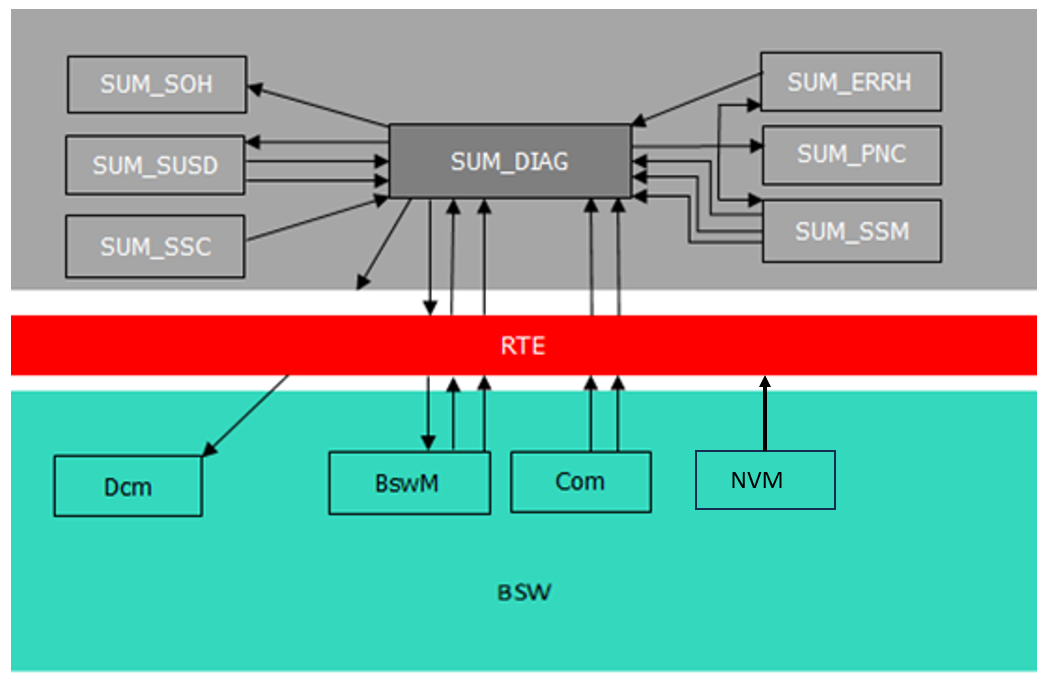
\includegraphics[width=1\textwidth]{images/Layers_definition.png}
	\caption{System layer overview.}
	\label{layer_overview}
\end{figure}
	
\section{References}
\input{generated/tables/references.tex}

\section{User Guide Revision History}
\input{generated/tables/rev_history.tex}